\chapter{Avaliação e Resultados} \label{chap:resultados}
\textbf{FALTA FAZER ESTE TEXTO}

A hipótese levantada no âmbito desta dissertação é que o uso de abstração em imagens que vão ser ser alvo de reconhecimento facial pode melhorar o processo de reconhecimento facial automático em imagens. Para a análise desta hipótese foi criado um sistema de reconhecimento facial automático em imagens, assim  como, escolhida uma biblioteca de imagens a analisar, tal como descrito em \ref{chap:visage}. Neste capítulo, é apresentada a metodologia de avaliação adotada para a análise da hipótese levantada, assim como do sistema de reconhecimento facial Visage e são também apresentados os resultados obtidos.



-Definição da coleção base a analisar

-Definição de quais os conjuntos de teste a criar a partir da coleção base

-Definição das experiências que se pretendem realizar e porquê

-Forma de avaliar e resultados dessas experiências

O desempenho de sistemas de reconhecimento facial pode ser analisado através de diferentes perspetivas, tal como introduzido na secção \ref{sec:problema} desta dissertação. A biblioteca LFW foi criada com o propósito inicial da análise do sub-problema de reconhecimento facial \textit{pair matching}, no qual o sistema deve decidir se duas faces representam ou não o mesmo indivíduo. No entanto, as características desta biblioteca, nomeadamente no que diz respeito à existência da anotação textual das pessoas presentes em cada imagem, à existência de apenas uma pessoa representada (de forma relevante) em cada imagem e ainda da normalização do formato das imagens, permitem que esta biblioteca possa ser utilizada com um esforço reduzido para o analise dos restantes sub-problemas de reconhecimento facial automático.

No âmbito desta dissertação temos em vista a realização de um conjunto de experiências descritas em \ref{sec:experiencias} e análise dos seus resultados através de duas perspetivas descritas nos pontos \ref{sec:avaliacao1} e \ref{sec:avaliacao2} a seguir. Uma vez que estas avaliações não se encontram enquadradas no paradigma de avaliação de \textit{pair matching}, para o qual a biblioteca LFW foi originalmente criada tornou-se necessário a criação de novos conjuntos de teste, os quais passamos a apresentar de seguida.

As imagens dos conjuntos de testes descritos em \ref{sec:conjuntos} foram sujeitas a um conjunto de tarefas de pré-processamento, descritas em \ref{sec:experiencias}, resultado na criação de um conjunto de galerias de imagens pré-processadas, as quais se encontram resumidas na tabela \ref{tab:colecoes}. Todas as galerias resultantes possuem as mesmas imagens, diferenciando-se apenas pelas tarefas de pré-processamento a que foram sujeitas.

Nesta secção encontram-se reportados os resultados da avaliação efetuada ao desempenho do sistema de reconhecimento facial Visage.

A qualidade do desempenho de um sistema de reconhecimento facial automático, assim como a satisfação dos seus utilizadores está intimamente relacionada com o fim para o qual o sistema foi criado. No âmbito desta dissertação, a avaliação do desempenho foi efetuada segundo duas perspetivas distintas, \textit{Closed-set Identification} e \textit{Image Retrieval}, as quais são apresentadas de seguida. A primeira constitui uma medida padrão de avaliação do desempenho de sistemas de reconhecimento facial automático, a segunda, pretende analisar o desempenho do sistema de um ponto de vista mais próximo de um provável caso de uso, neste caso, \textit{Image Retrieval}.


\section{Conjuntos de Teste}  \label{sec:conjuntos}

Na avaliação de sistemas de reconhecimento facial automáticos designam-se de \textit{amostras biométricas} as capturas de características de uma pessoa que permitem efetuar o seu reconhecimento. Dependendo do sistema, as amostras biométricas podem ser apenas uma imagem, um conjunto de imagens, ou um vídeo. No projeto Visage as amostras biométricas de um indivíduo são constituídas por um conjunto de imagens, um exemplo de amostras biométricas de um indivíduo para a biblioteca LFW-a pode encontra-se representado nas figuras \ref{fig:galeria}  e \ref{fig:provas}. Designam-se ainda de \textit{provas} as amostras biométricas apresentadas ao sistema para serem reconhecidas.

Para a avaliação efetuada foram criados 4 conjuntos de teste. Todos os conjuntos possuem um total de 1180 imagens, correspondentes a amostras biométricas de 59 pessoas diferentes, existindo 20 imagens por cada pessoa presente em cada conjunto. Dessas imagens foram ainda criados dois conjuntos de dados: conjunto $\mathscr{G}$, designado de galeria de treino e conjunto $\mathscr{P}$, designado de provas.

\begin{figure}
        \centering
        \begin{subfigure}[b]{0.2\textwidth}
                \centering
                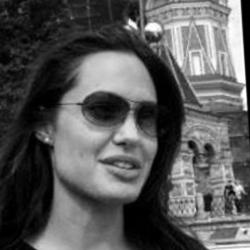
\includegraphics[width=\textwidth]{angelina/1}
        \end{subfigure}%
        ~ %add desired spacing between images, e. g. ~, \quad, \qquad etc.
        \begin{subfigure}[b]{0.2\textwidth}
                \centering
                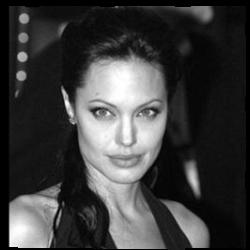
\includegraphics[width=\textwidth]{angelina/2}
        \end{subfigure}
        ~
        \begin{subfigure}[b]{0.2\textwidth}
                \centering
                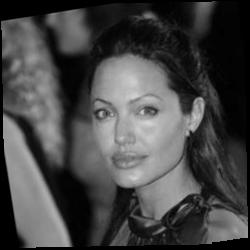
\includegraphics[width=\textwidth]{angelina/3}
        \end{subfigure}%
        ~ %add desired spacing between images, e. g. ~, \quad, \qquad etc.
        \begin{subfigure}[b]{0.2\textwidth}
                \centering
                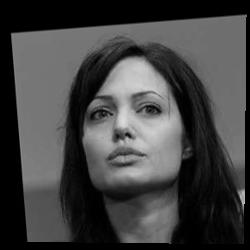
\includegraphics[width=\textwidth]{angelina/4}
        \end{subfigure}
%

        \begin{subfigure}[b]{0.2\textwidth}
                \centering
                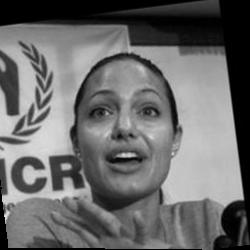
\includegraphics[width=\textwidth]{angelina/5}
        \end{subfigure}%
        ~ %add desired spacing between images, e. g. ~, \quad, \qquad etc.
        \begin{subfigure}[b]{0.2\textwidth}
                \centering
                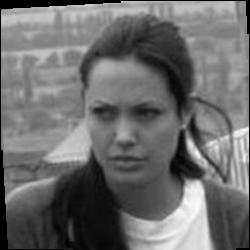
\includegraphics[width=\textwidth]{angelina/6}
        \end{subfigure}
        ~
        \begin{subfigure}[b]{0.2\textwidth}
                \centering
                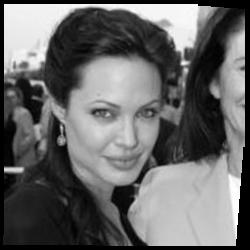
\includegraphics[width=\textwidth]{angelina/7}
        \end{subfigure}%
        ~ %add desired spacing between images, e. g. ~, \quad, \qquad etc.
        \begin{subfigure}[b]{0.2\textwidth}
                \centering
                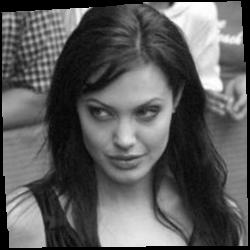
\includegraphics[width=\textwidth]{angelina/8}
        \end{subfigure}
%
        \begin{subfigure}[b]{0.2\textwidth}
                \centering
                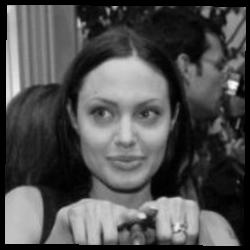
\includegraphics[width=\textwidth]{angelina/9}
        \end{subfigure}%
        ~ %add desired spacing between images, e. g. ~, \quad, \qquad etc.
        \begin{subfigure}[b]{0.2\textwidth}
                \centering
                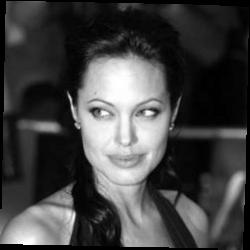
\includegraphics[width=\textwidth]{angelina/10}
        \end{subfigure}
        ~
        \begin{subfigure}[b]{0.2\textwidth}
                \centering
                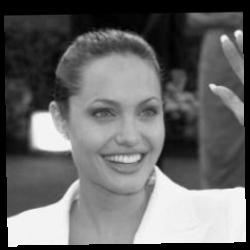
\includegraphics[width=\textwidth]{angelina/11}
        \end{subfigure}%
        ~ %add desired spacing between images, e. g. ~, \quad, \qquad etc.
        \begin{subfigure}[b]{0.2\textwidth}
                \centering
                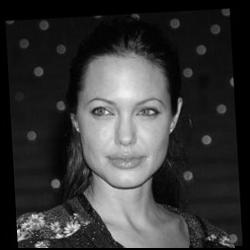
\includegraphics[width=\textwidth]{angelina/12}
        \end{subfigure}
%
        \begin{subfigure}[b]{0.2\textwidth}
                \centering
                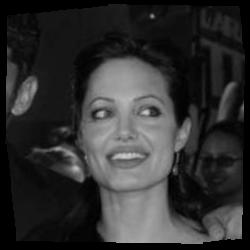
\includegraphics[width=\textwidth]{angelina/13}
        \end{subfigure}%
        ~ %add desired spacing between images, e. g. ~, \quad, \qquad etc.
        \begin{subfigure}[b]{0.2\textwidth}
                \centering
                
\includegraphics[width=\textwidth]{angelina/14}
        \end{subfigure}
        ~
        \begin{subfigure}[b]{0.2\textwidth}
                \centering
                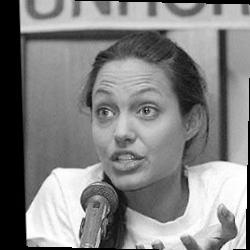
\includegraphics[width=\textwidth]{angelina/15}
        \end{subfigure}%
        ~ %add desired spacing between images, e. g. ~, \quad, \qquad etc.
        \begin{subfigure}[b]{0.2\textwidth}
                \centering
                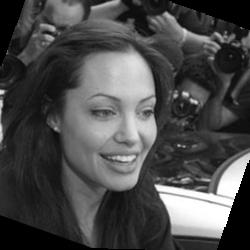
\includegraphics[width=\textwidth]{angelina/16}
        \end{subfigure}
        \caption{Exemplo de imagens do conjunto $\mathscr{G}$ para o sujeito Angelina Jolie}
        \label{fig:galeria}        
\end{figure}

A galeria de treino, $\mathscr{G}$, é constituída por 80\% das imagens de cada pessoa (16 imagens por pessoa), sendo as suas imagens utilizadas como amostras biométricas para o treino do sistema de reconhecimento facial. Um exemplo das imagens presentes na galeria de treino para o sujeito Angelina Jolie pode ser visto na figura \ref{fig:galeria}.

\begin{figure}
        \centering
        \begin{subfigure}[b]{0.2\textwidth}
                \centering
                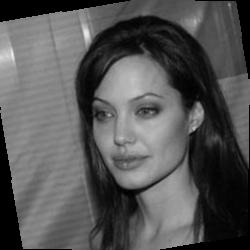
\includegraphics[width=\textwidth]{angelina/17}
        \end{subfigure}%
        ~ %add desired spacing between images, e. g. ~, \quad, \qquad etc.
        \begin{subfigure}[b]{0.2\textwidth}
                \centering
                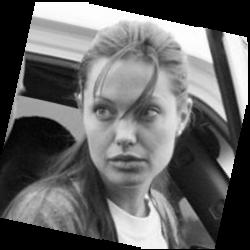
\includegraphics[width=\textwidth]{angelina/18}
        \end{subfigure}
        ~
        \begin{subfigure}[b]{0.2\textwidth}
                \centering
                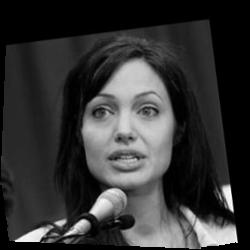
\includegraphics[width=\textwidth]{angelina/19}
        \end{subfigure}%
        ~ %add desired spacing between images, e. g. ~, \quad, \qquad etc.
        \begin{subfigure}[b]{0.2\textwidth}
                \centering
                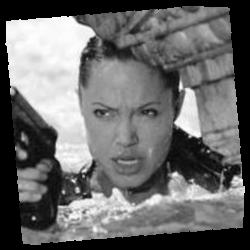
\includegraphics[width=\textwidth]{angelina/20}
        \end{subfigure}
        \caption{Exemplo de imagens do conjunto $\mathscr{P}$ para o sujeito Angelina Jolie}
        \label{fig:provas}   
\end{figure}

O conjunto $\mathscr{P}$ contem os restantes 20\% das imagens de cada pessoa (4 imagens por pessoa) e, tal como o seu nome indica, as suas imagens são utilizadas para a avaliação do sistema desenvolvido. Um exemplo das imagens presentes nas provas para o sujeito Angelina Jolie pode ser visto na figura \ref{fig:provas}.

A diferença existente entre os quatro conjuntos criados encontras-se relacionada com as imagens incluídas na galeria de treino e nas provas, sendo que estas diferem de forma aleatória entre os quatro conjuntos. A criação de 4 conjuntos com igual tamanho mas diferentes imagens de treino e teste tem em vista analisar o desempenho do sistema com diferentes galerias, de forma a determinar se existe uma variação significativa dos resultados obtidos em cada galeria.

\section{Pré-processamento} \label{sec:experiencias}
O módulo de reconhecimento facial, \textit{Face Recognizer}, disponibilizado pela plataforma \textit{OpenCV}, constituiu uma base sólida para o desenvolvimento do sistema de reconhecimento facial \textit{Visage}, contudo, de modo a tornar este sistema mais completo e versátil, revelou-se necessário adapta-lo e expandir as suas capacidades, nomeadamente através da aplicação de uma cadeia de pré-processamento às imagens existentes \footnote{a qual se encontra ilustrada na figura \ref{fig:preprocessamento}}. A evolução do sistema desenvolvido foi efetuada de forma gradual e iterativa, e culminou na construção de um conjunto de galerias de imagens, analisadas através de um grupo de experiências que permitem tirar conclusões acerca dos efeitos das diversas etapas de pré-processamento realizadas e da contribuição de cada uma delas para a melhoria do desempenho do sistema criado. 

Todas as galerias criadas possuem as imagens contidas nos conjuntos de teste definidos em \ref{sec:conjuntos}, diferenciando-se pelos diferentes passos de pré-processamento a que as imagens foram sujeitas. De notar que, tal  como representado em \ref{fig:preprocessamento}, o pré-processamento das imagens é efetuado antes da aplicação da máscara nas mesmas, de forma a não afetar os resultados obtidos nas tarefas de pré-processamento. Na tabela \ref{tab:colecoes} encontram-se resumidas as galerias resultantes do conjunto de experiências efetuadas, as quais se encontram descritas pormenorizadamente de seguida.

\subsection{Deteção e segmentação da face}
Na revisão efetuada ao estado da arte do reconhecimento facial em imagens destacou-se a importância da resolução de um conjunto de sub-problemas específicos para um reconhecimento facial eficaz (ver \ref{sec:sub-problemas}), nomeadamente a deteção e segmentação das faces existentes numa imagem. Para a resolução deste problema, foi implementado o módulo de deteção facial descrito em \ref{chap:facedetector}. Na implementação deste módulo revelou-se necessário a avaliação de diferentes alternativas relativamente à forma como é efetuada a segmentação da face da restante imagem, assim como a determinação do impacto dessa segmentação. 

Após uma análise das diferente alternativas existentes, e através de alguns teste intermédios realizados durante o período de desenvolvimento, foram então criadas as galerias de imagens Original, figura \ref{fig:original}; Cropped, figura \ref{fig:cropped}; e Masked, figura \ref{fig:masked}. A primeira, é constituída pelas imagens originais da biblioteca LFW-a e permite estabelecer uma base de comparação entre as imagens segmentadas e as imagens originais. A galeria cropped é composta por um conjunto de imagens onde as faces foram detetadas e segmentadas pelo detetor facial implementado e descrito no capítulo \ref{chap:facedetector}. A terceira e última galeria criada possui as mesmas imagens da galeria Cropped, sobre as quais foi posteriormente aplicada uma máscara elíptica de modo a diminuir a presença de fundo nas imagens recortadas.

\subsection{Normalização do Contraste}
A normalização das imagens em termos de contraste é passo comum e essencial à maioria dos sistemas de reconhecimento facial automático modernos, tal como destacado no capítulo \ref{chap:reco} desta dissertação. Assim sendo, no decorrer do desenvolvimento do sistema de reconhecimento facial Visage, revelou-se também importante analisar o qual o impacto da normalização do contraste nas imagens utilizadas, assim como qual a melhor forma de efetuar a sua normalização. Foram então estudadas três formas distintas de efetuar a normalização do contraste, as quais são apresentadas de seguida:

\begin{description}
\item[\textit{Contrast Streching}]
A técnica de \textit{Contrast Streching}, também designada por alguns autores simplesmente de normalização, consiste numa tentativa de alargar a gama de valores utilizados para codificar a intensidade de uma imagem de forma a que seja utilizada toda a gama de valores possíveis. Nesta avaliação as imagens utilizadas encontram-se convertidas para tons de cinzento, pelo que a normalização efetuada consiste num mapeamento linear dos valores originais para uma gama de intensidade entre 0 e 255. Da aplicação da técnica de contrast streching às imagens presentes nos conjuntos de teste descritos anteriormente resultou a criação da galeria Normalized. Um exemplo de uma imagem dessa galeria pode ser visualizado na imagem \ref{fig:normalized}.
\end{description}

\begin{description}
\item[Equalização Histograma]
O histograma de uma imagem descreve a distribuição estatística dos níveis de intensidade de uma imagem, neste caso concreto dos níveis de cinzento, em função do seu número de pixeis. A equalização do histograma de uma imagem consiste no mapeamento das variações da escala de cinzentos de forma a que o histograma resultante se aproxime de uma outra distribuição, mais alargada e idealmente uniforme na distribuição dos valores de intensidade da imagem. Este procedimento parte do princípio de que a qualidade da imagem é uniforme em toda a imagem, aplicando um mapeamento similar a toda a imagem \cite{Bradski2008}. As imagens normalizadas através da equalização simples do histograma encontram-se representadas na galeria Equalized e um exemplo das mesmas pode ser visto na figura \ref{fig:equalized}.
\end{description}

\begin{description}
\item[\textit{CLAHE}]
\textit{Contrast limited adaptive histogram equalization (CLAHE)} procura ultrapassar as limitações da equalização de contraste, através de uma abordagem local ao problema de normalização do histograma de uma imagem. Ao contrário da abordagem tradicional apresentada acima, esta técnica tem em conta a intensidade de um conjunto de pixeis e dos seus vizinhos para a normalização do seu contraste e não a intensidade de toda a imagem. Para além disso, tal como o seu nome indica, esta abordagem incluí ainda um limite para o qual a equalização do histograma é realizada, evitando assim a o mapeamento demasiado agressivo quando duas escalas de intensidade dispares se encontram na mesma região \cite{Reza2004}. Na imagem \ref{fig:clahe} encontra-se representada uma imagem da galeria CLAHE, resultante da normalização das imagens dos conjuntos de teste através da técnica CLAHE.
\end{description}

\subsection{Abstração Imagens}
A terceira experiência visa analisar o impacto da abstração de imagens no reconhecimento.

Gaussian Blur

Bilateral

Anisotropic Kuwahara

\begin{figure}
        \centering
        \begin{subfigure}[b]{0.2\textwidth}
                \centering
                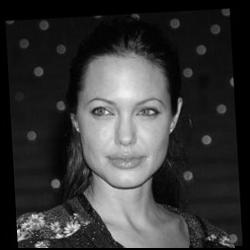
\includegraphics[width=\textwidth]{angelina/Angelina_Jolie_0006}
                \caption{Original}
                \label{fig:original} 
        \end{subfigure}%
%

        \begin{subfigure}[b]{0.2\textwidth}
                \centering
                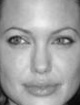
\includegraphics[width=\textwidth]{angelina/Angelina_Jolie_0006_cropped}
                \caption{Cropped}
                \label{fig:cropped} 
        \end{subfigure}
        ~ ~
        \begin{subfigure}[b]{0.2\textwidth}
                \centering
                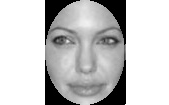
\includegraphics[width=\textwidth]{angelina/Angelina_Jolie_0006_masked}
                \caption{Masked}
                \label{fig:masked}
        \end{subfigure}%
%

        \begin{subfigure}[b]{0.2\textwidth}
                \centering
                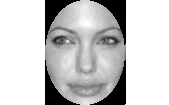
\includegraphics[width=\textwidth]{angelina/Angelina_Jolie_0006_normalized}
                \caption{Normalized}
                \label{fig:normalized} 
        \end{subfigure}
        ~ ~
        \begin{subfigure}[b]{0.2\textwidth}
                \centering
                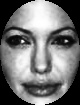
\includegraphics[width=\textwidth]{angelina/Angelina_Jolie_0006_equalized}
                \caption{Equalized}
                \label{fig:equalized}
        \end{subfigure}
        ~ ~
        \begin{subfigure}[b]{0.2\textwidth}
                \centering
                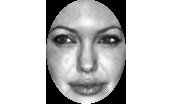
\includegraphics[width=\textwidth]{angelina/Angelina_Jolie_0006_CLAHE}
                \caption{CLAHE}
                \label{fig:clahe}
        \end{subfigure}
        \caption{Exemplo dos vários pré-processamentos disponíveis.}
        \label{fig:galeriaspreprocessadas}   
\end{figure}


\begin{center}
\begin{table}
	\caption{Galerias criadas após pré-processamento.}
	\begin{center}
    \begin{tabular}{l|cccc|c}
    \hline\hline
    Designação & Recortada   & Normalização           & Filtro Abstração & Máscara & Exemplo \\
	\hline
    Original   &   -         & -                      & -                &   -     & \ref{fig:original} \\
	~ & ~ & ~ & ~ & ~ & ~\\
    Cropped    & Sim         & -                      & -                &   -     & \ref{fig:cropped}  \\
    Masked     & Sim         & -                      & -                & Sim     & \ref{fig:masked}  \\
	~ & ~ & ~ & ~ & ~ & ~\\
    Normalized & Sim         & Constrast Streching    & -                & Sim     & \ref{fig:normalized}  \\
    Equalized  & Sim         & Histogram Equalization & -                & Sim     & \ref{fig:equalized}  \\
    CLAHE      & Sim         & CLAHE                  & -                & Sim     & \ref{fig:clahe}  \\
	~ & ~ & ~ & ~ & ~ & ~\\
    Bilateral  & Sim         & Histogram Equalization & Bilateral Filter & Sim       \\
    Gaussian   & Sim         & Histogram Equalization & Gaussian Filter  & Sim       \\
    \hline\hline
    \end{tabular}
	\label{tab:colecoes}
	\end{center}
\end{table}
\end{center}


\section{Avaliação \textit{Closed-Set Identification}} \label{sec:avaliacao1}
Tal como introduzido na secção \ref{sec:problema}, o paradigma de \textit{closed-set identification}, constitui um sub-problema de identificação em que uma prova é apresentada ao sistema e pretende-se que este devolva a identidade da pessoa presente na imagem. Neste caso particular do problema de identificação, todas as provas apresentadas possuem uma correspondência na galeria, em oposição ao caso geral de identificação, no qual pode ou não haver uma correspondência.

A avaliação \textit{closed-set} é uma medida padrão de avaliação do desempenho em sistemas de reconhecimento facial automático, tendo sido utilizada em diversas avaliações efetuadas, nomeadamente nas avaliações FERET e FRVT apresentadas na revisão do estado da arte desta dissertação (ver \ref{chap:reco}). A utilização de um conjunto fechado de imagens permite uma análise detalhada do desempenho de um algoritmo permitindo responder à pergunta "a identificação correta encontra-se nos primeiros $n$ resultados?" em vez de apenas " o primeiro resultado é o correto?".

\subsection{Metodologia Avaliação}
Para cada conjunto de teste descrito em \ref{sec:conjuntos}, seja $\mathscr{G}$ a sua galeria de treino, em que $\mathscr{G} = \{g_1, ..., g_N\}$ e seja $\mathscr{P}$ o conjunto das suas provas, em que $\mathscr{P} = \{p_1, ..., p_N\}$. Quando uma prova $p_j$ é apresentada ao sistema, essa prova é então comparada a cada amostra biométrica $g_i$ da galeria, resultando dessa comparação o respetivo índice de similaridade (\textit{similarity score}), $s_{ij}$. Este índice é designado de $match$ $score$, caso $g_i$ e $p_j$ sejam amostras da mesma pessoa, caso não o sejam é designado de $nonmatch$ $score$. Quanto menor o índice de similaridade, maior é a probabilidade das imagens comparadas pertencerem à mesma pessoa, sendo que o melhor valor possível para o índice de similaridade de um $match$ $score$ é zero.

Na identificação de $p_j \in \mathscr{P}$, em primeiro lugar são calculados os índices de similaridade para todas as amostras na galeria $\mathscr{G}$, sendo posteriormente ordenados os seus resultados. O ranking de $p_j$, $r_{p_j}$, é igual a $n$, se o seu $match$ $score$ corresponde ao enésimo menor índice de similaridade. A taxa de identificação para o ranking $n$, $T_{I}(n)$, corresponde à fração de provas com ranking $n$ ou menor do que $n$, ou seja:
\begin{equation}
T_{I}(n) = \frac{|C(n)|}{|\mathscr{P}|} \times 100
\end{equation}
Em que $|C(n)|$ é número de provas com ranking $n$, ou menor do que $n$, e $|\mathscr{P}|$ o número de provas existentes em $\mathscr{P}$.

A $T_{I}(n)$ é calculada para todos os rankings entre 1 e 30. Dentro desse intervalo, os primeiros níveis de ranking apresentam uma maior variação na percentagem de pessoas identificadas, revelando-se assim mais significativos para a análise do desempenho do sistema.

A avaliação é efetuada através da análise do desempenho dos três algoritmos disponíveis em cada uma das galerias de imagens pré-processadas, encontrando-se os resultados obtidos agrupados num conjunto de três experiências, cada uma dedicada a analisar a variação do comportamento do sistema dado um problema específico. A divisão entre imagens de treino e teste de cada galeria é efetuada segundo os quatro conjuntos de testes criados, sendo cada galeria avaliada em cada um dos quatro conjuntos de teste existentes e posteriormente calculada a média dos resultados obtidos.

A média dos resultados obtidos encontra-se representada em um gráfico do tipo \textit{Cumulative match score} (CMS). Um gráfico do tipo CMS representa $T_{I}(n)$ como uma função de ranking $n$. No eixo horizontal encontra-se representado o ranking e no eixo vertical encontra-se representada a respetiva taxa de identificação, um exemplo de um gráfico CMS pode ser visto em \ref{fig:exp1_comaparacao}.

\subsection{Resultados Experiência 1 : Análise do impacto da segmentação das faces}

\begin{figure}[p]
        \centering
        \begin{subfigure}[b]{0.58\textwidth}
                \centering
                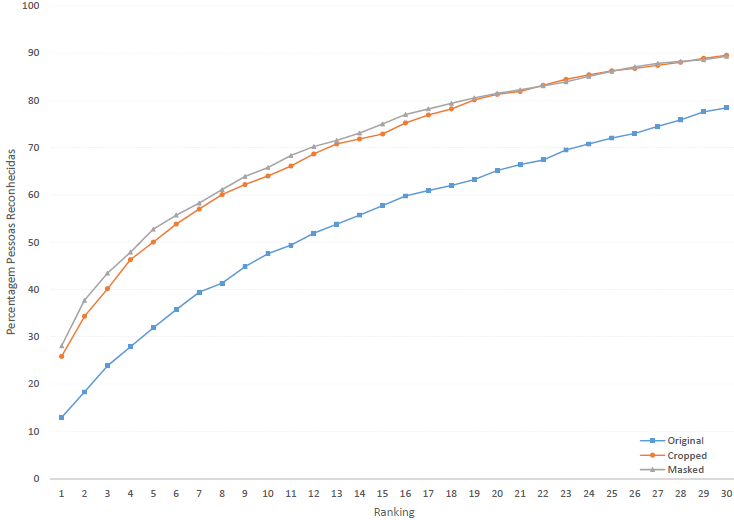
\includegraphics[width=\textwidth]{resultados/original_cropped_masked_eigen}
                \caption{Eigenfaces}
                \label{fig:original_cropped_masked_eigen}
        \end{subfigure}%

        \begin{subfigure}[b]{0.58\textwidth}
                \centering
                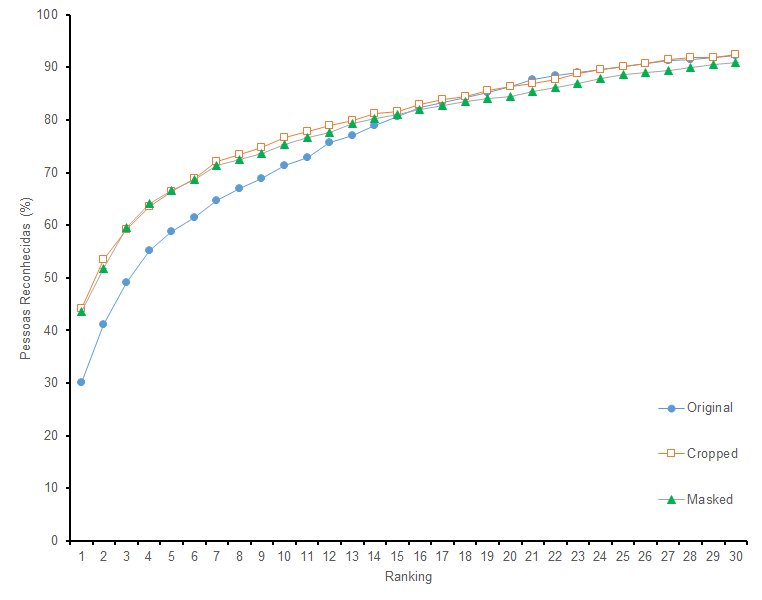
\includegraphics[width=\textwidth]{resultados/original_cropped_masked_fisher}
                \caption{Fisherfaces}
                \label{fig:original_cropped_masked_fisher}
        \end{subfigure}

        \begin{subfigure}[b]{0.58\textwidth}
                \centering
                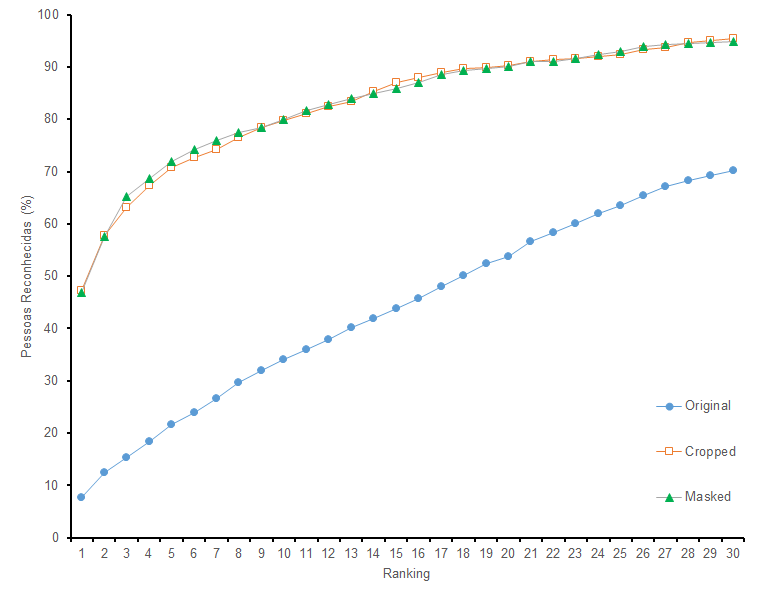
\includegraphics[width=\textwidth]{resultados/original_cropped_masked_lbph}
                \caption{LBPH}
                \label{fig:original_cropped_masked_lbph}
        \end{subfigure}
        \caption{Desempenho algoritmos Eigenfaces, Fisherfaces e LBPH para os conjuntos Original, Cropped e Masked}
        \label{fig:original_cropped_masked}
\end{figure}

Esta experiência visa analisar o impacto da segmentação das faces presentes na imagem do fundo existente nas mesmas, assim como determinar qual, de entre duas alternativas, a melhor forma de segmentar essa mesma face. Os resultados obtidos podem ser visualizados na figura \ref{fig:original_cropped_masked}, onde se encontram ilustrada a performance dos algoritmos, \textit{Eigenfaces}, \textit{Fisherfaces} e \textit{LBPH}, nos três conjuntos criados especialmente para esta experiência, os quais se encontram descritos mais pormenorizadamente em \ref{sec:experiencias}.

Após a analise dos resultados obtidos na experiência 1, nomeadamente através da comparação das taxa de identificação de ranking 1 dos conjuntos Cropped e Masked com o conjunto Original, verifica-se que a segmentação das faces presentes nas imagens originais produz uma melhoria efetiva dos resultados obtidos, traduzindo-se num aumento de cerca de 12\%, 14\% e 40\% para os algoritmos \textit{Eigenfaces}, \textit{Fisherfaces} e \textit{LBPH}, respetivamente.

Uma análise mais aprofundada desses resultados, demonstra ainda que, no caso dos algoritmos \textit{Eigenfaces} e \textit{LBPH}, a diferença na taxa de identificação entre as imagens originais (conjunto Original) e as imagens segmentadas (conjuntos Cropped e Masked) é significativa e relativamente constante nos vários níveis para os quais a taxa de deteção se encontra reportada. Por outro lado, no caso do algoritmo \textit{Fisherfaces}, apesar da diferença significativa no número de imagens corretamente identificadas nos primeiros níveis, a partir do ranking 15, todos os conjuntos de imagens obtém uma taxa de identificação similar, e com uma progressão semelhante. Esta aproximação no número de caras corretamente identificadas nos rankings mais elevados pode ser explicada pela existência de informação no fundo das imagens, a qual poderá ser utilizada pelo próprio algoritmo para a identificação das mesmas, ao invés da utilização da face contida na imagem, reforçando assim a importância da extração do fundo contido nas imagens originais.

Por outro lado, note-se ainda que, apesar do impacto positivo da segmentação das imagens nos três algoritmos testados, o impacto desta segmentação varia significativamente conforme o algoritmo utilizado, sendo que o \textit{Fisherfaces} é o que revela resultados mais constantes independentemente da manipulação efetuada nas imagens e o algoritmo \textit{LBPH} o que regista uma maior melhoria desses mesmos resultados.

Ao nível da diferença entre as imagens apenas segmentadas (conjunto Cropped) e as imagens com máscara (conjunto Masked), é possível verificar que ambas possuem resultados semelhantes, sendo que a maior diferença foi detetada no algoritmo \textit{Eigenfaces}, onde as imagens com máscara demonstraram um desempenho ligeiramente superior, como é possível verificar pelas $T_{I}(2)$ de 43,4\% e 40,1\% para as imagens com máscara e recortadas, respetivamente. Apesar da diferença registada ser muito significativa, a existência de uma máscara garante uma extração de uma maior quantidade de fundo das imagens, permitindo assim uma maior confiança dos resultados obtidos, no sentido em que se reduz o perigo de identificação pelas características do fundo da imagem e não das caraterísticas faciais presentes na mesma. 

\begin{figure}[ht]
  \begin{center}
    \leavevmode
    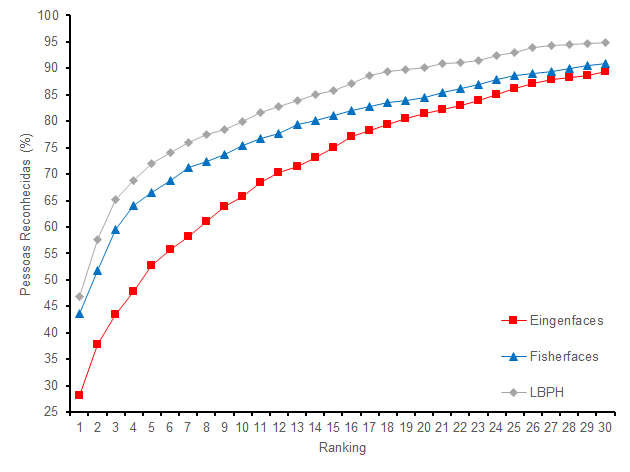
\includegraphics[width=0.6\textwidth]{resultados/exp1_comparacao}
    \caption{Comparação do desempenho dos três algoritmos implementados para o conjunto Masked}
    \label{fig:exp1_comaparacao}
  \end{center}
\end{figure}

Finalmente, através da análise do gráfico \ref{fig:exp1_comaparacao}, é possível concluir que ao nível dos algoritmos utilizados o algoritmo \textit{LBPH} obtém resultados globalmente melhores, ao passo que o algoritmo \textit{Eingefaces} obtém os piores resultados. Esta diferença verifica-se quer nos rankings inferiores, quer nos superiores, sendo menor quanto maior é o ranking utilizado, como é possível verificar pelas taxas de identificação de ranking 1 de 46,8\% e 28,1\%, no conjunto Masked, para os algoritmos \textit{LBPH} e \textit{Eigenfaces}, respetivamente, e pelas taxas de identificação de ranking 30 de 94,9\% e 89,3\%, para os mesmos algoritmos no mesmo conjunto.

\subsection{Resultados Experiência 2: Impacto da Normalização do Contraste}
\begin{figure}[p]
        \centering
        \begin{subfigure}[b]{0.58\textwidth}
                \centering
                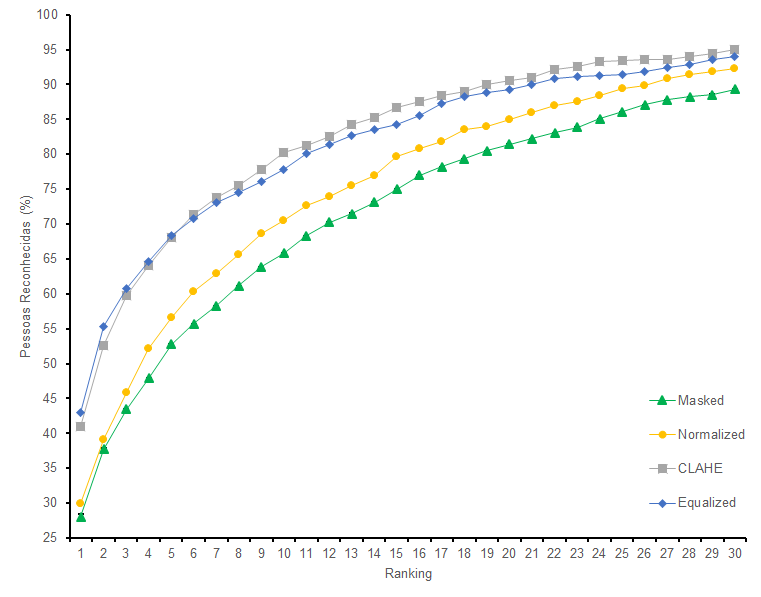
\includegraphics[width=\textwidth]{resultados/Exp_2_eigen}
                \caption{Eigenfaces}
                \label{fig:masked_normalized_equalized_clahe_eigen}
        \end{subfigure}%

        \begin{subfigure}[b]{0.58\textwidth}
                \centering
                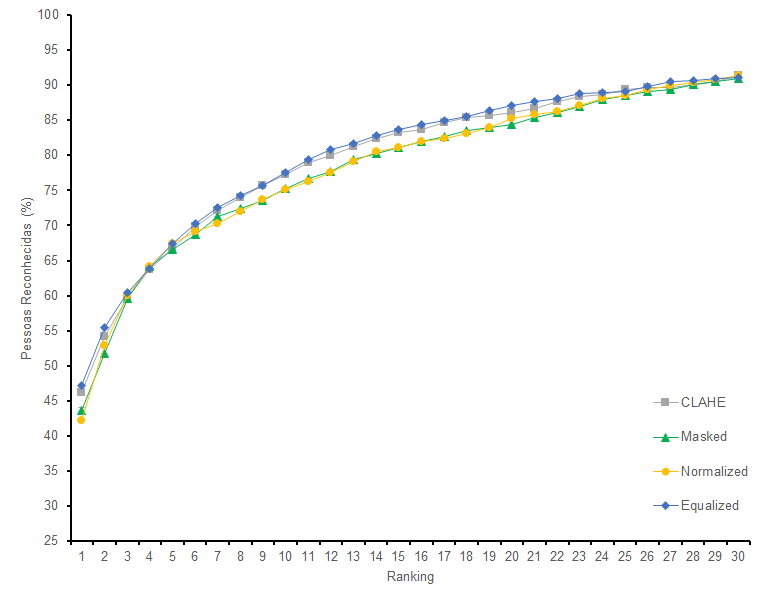
\includegraphics[width=\textwidth]{resultados/Exp_2_fisher}
                \caption{Fisherfaces}
                \label{fig:masked_normalized_equalized_clahe_fisher}
        \end{subfigure}

        \begin{subfigure}[b]{0.58\textwidth}
                \centering
                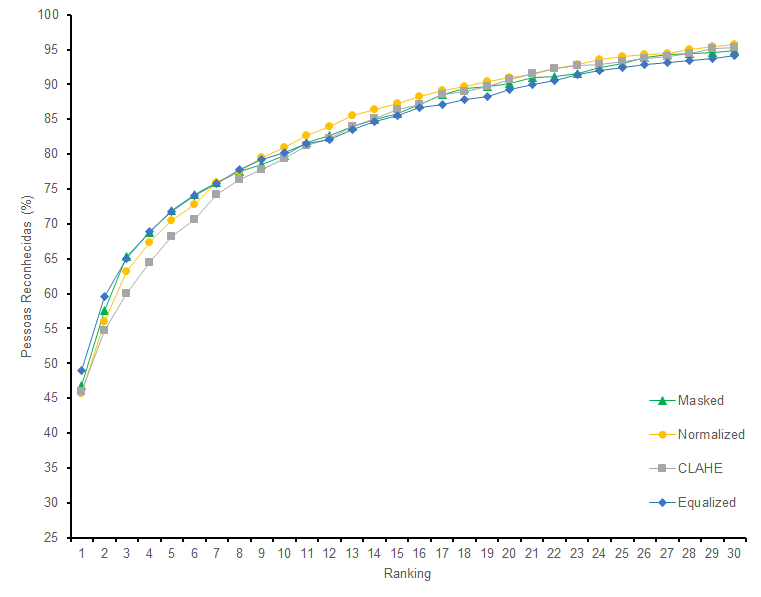
\includegraphics[width=\textwidth]{resultados/Exp_2_lbph}
                \caption{LBPH}
                \label{fig:masked_normalized_equalized_clahe_lbph}
        \end{subfigure}
        \caption{Desempenho algoritmos Eigenfaces, Fisherfaces e LBPH para os conjuntos Normalized, Equalized e CLAHE}
        \label{fig:exp2}
\end{figure}

A aquisição de imagens em condições não controladas pode resultar na obtenção de fotografias com um contraste reduzido e níveis de iluminação muito distintos. De forma a ultrapassar este problema, a normalização do contraste de uma imagem é uma tarefa comum nos sistemas de reconhecimento faciais modernos. Nesta experiência pretendemos analisar qual o impacto da normalização do contraste de uma imagem nos diferentes algoritmos implementados, assim como determinar qual a melhor de entre três técnicas distintas implementadas, através da analise do desempenho do sistema em três galerias previamente normalizadas com cada uma dessas técnicas (ver \ref{sec:experiencias}).

Na figura \ref{fig:exp2} é possível visualizar os resultados para obtidos para o desempenho do sistema nas galerias Normalized, Equalized e CLAHE, correspondentes às três técnicas de normalização \textit{contrast stretching}, equalização histograma e CLAHE, respectivamente. Nos gráficos da figura \ref{fig:exp2} encontra-se ainda representados os resultados obtidos para o conjunto Masked, utilizado na experiência 1, o qual serve de referência para a comparação entre os conjuntos não normalizados e os conjuntos normalizados.

Como é possível concluir pela observação da figura \ref{fig:exp2}, a normalização das imagens apresenta resultados globalmente melhores do que os obtidos para conjuntos não normalizados. O impacto obtido varia, no entanto, consideravelmente conforme o algoritmo utilizado, sendo que o maior impacto é registado para o algoritmo Eigenfaces, onde existe uma melhoria na ordem dos 15.0\% na percentagem de pessoas reconhecidas no primeiro nível do ranking, quando comparadas as galerias Masked e Equalized. Os algoritmos \textit{Fisherfaces} e \textit{LBPH} mostram uma diferença máxima de apenas 3.8\% e 2.2\% entre os conjuntos Masked e Equalized, pelo que é possível concluir que estes algoritmos possuem uma maior resistência aos efeitos da iluminação no desempenho quando comparados com o algoritmo \textit{Eigenfaces} \footnote{A pouca variação obtida neste dois últimos algoritmos vai de acordo com o defendido por investigações anteriores realizadas por \cite{ahonen2004face}.}.

Ao nível das três técnicas utilizadas é possível concluir que as duas variantes de equalização do histograma possuem os resultados mais satisfatórios. A equalização simples do histograma, conjunto Equalized, tem tendência a demonstrar resultados melhores para os primeiros níveis de ranking, sendo posteriormente igualada ou até ultrapassada pela técnica CLAHE nos níveis mais superiores. Uma vez que os primeiros níveis de ranking incluem a informação mais significativa para a maioria dos utilizadores de sistemas de reconhecimento facial automático, consideramos que o desempenho da equalização do histograma das imagens possuí resultados mais relevantes para a utilização no sistema de reconhecimento facial Visage do que a técnica \textit{CLAHE}.

\begin{figure}[ht]
  \begin{center}
    \leavevmode
    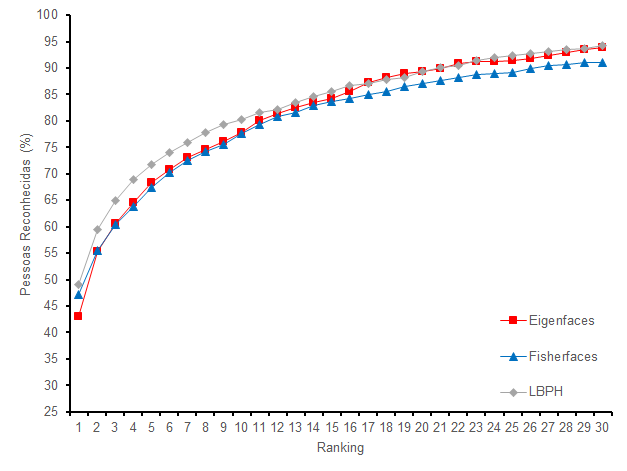
\includegraphics[width=0.6\textwidth]{resultados/exp2_comparacao}
    \caption{Comparação do desempenho dos três algoritmos implementados para o conjunto Equalized}
    \label{fig:exp2_comaparacao}
  \end{center}
\end{figure}

Finalmente, a análise comparativa dos resultados obtidos para os três algoritmos implementados, ilustrada pelo gráfico \ref{fig:exp2_comaparacao}, permite concluir que após a normalização do histograma das imagens o desempenho dos algoritmos apresenta uma diferença muito menor do que a registada anteriormente e ilustrada pelo gráfico \ref{fig:exp1_comaparacao}. Nesta experiência o algoritmo LBPH continua a ser o algoritmo com melhor desempenho, registando no entanto uma diferença de apenas 1.8\% e 6.0\% para os algoritmos \textit{Fisherfaces} e \textit{Eigenfaces}, respetivamente, na taxa de identificação de ranking 1 no conjunto Equalized. De notar ainda que, a partir do segundo nível do ranking, o algoritmo  \textit{Eigenfaces} possui uma taxa de identificação idêntica ao valores obtidos pela algoritmo \textit{Fisherfaces}, ultrapassando o desempenho do segundo, a partir do ranking 11. Esta grange evolução no desempenho, notada para o algoritmo \textit{Eigenfaces}, em contraste com a ligeira melhoria obtida pelos restantes denota a complexidade associada ao problema de reconhecimento facial automático, nomeadamente no que diz respeito à forma como diferentes fatores afetam de forma diferenciada diferentes algoritmos e diferentes conjuntos de dados.

\subsection{Resultados Experiência 3}

\section{Avaliação \textit{Image Retrieval}} \label{sec:avaliacao2}
A metodologia de avaliação proposta na secção \ref{sec:avaliacao1} desta dissertação permite-nos efetuar uma avaliação qualitativa do desempenho do sistema de reconhecimento facial criado, assim como dos diferentes algoritmos implementados, através de uma medida padrão para a avaliação de sistemas de reconhecimento facial automáticos. Nesta segunda avaliação propomos a avaliação do desempenho do sistema de um ponto de vista centrado num possível caso de uso do mesmo: \textit{Image Retrieval}.

A área de recuperação de informação multimédia regista atualmente uma importância crescente, resultado do elevado número de conteúdos produzidos, assim como do elevado número de dispositivos de partilha disponíveis, tal como destacado no estado da arte desta dissertação. Desta forma, a recuperação de informação multimédia e em particular a área de \textit{Image Retrieval} representa uma das áreas com maior potencial para a utilização do sistema de reconhecimento facial criado.

Para uma dada imagem contendo uma face, o sistema Visage é capaz de detetar a face presente na imagem e apresentar uma lista ordenada de possíveis entidades que se encontram representadas nessa imagem. Com base neste sistema é possível desenvolver aplicações de \textit{image retrieval} capazes de encontrar fotos de uma personalidade específica ou apresentar, para uma foto de rosto fornecida pelo utilizador, a celebridade ou figura pública mais parecida.

\subsection{Metodologia Avaliação}
Em recuperação de informação multimédia designa-se de \textit{precisão} a fração de documentos relevantes do total de documentos retornados por uma pesquisa. Ao analisar a precisão podem ser analisados todos os documentos relevantes ou apenas os $n$ documentos mais relevantes, designado-se nessa situação de \textit{precisão a n}.

No sistema de reconhecimento facial criado, para uma dada imagem é apresentada uma lista de possíveis entidades que se encontram representadas nessa imagem, em que o primeiro resultado representa a entidade com maior probabilidade de estar presente na imagem e em que cada entidade aparece uma única vez na lista de resultados possíveis. Caso se pretenda efetuar a identificação de uma personalidade existe apenas um resultado verdadeiramente relevante na lista de resultados obtida, pelo que a medida de \textit{precisão a n} utilizada em recuperação de informação multimédia não é válida para a avaliação efetuada nesta secção.

Para avaliação do desempenho do sistema do ponto de vista de \textit{image retrieval} foi então criada a medida \textit{precisão na galeria} (PG). A \textit{precisão na galeria} resulta da adaptação da precisão de recuperação de informação multimédia ao caso particular do sistema de reconhecimento facial automático desenvolvido. Considerando a definição de ranking de uma prova apresentada em \ref{sec:avaliacao1}, a \textit{precisão na galeria} de $p_j$, $PG_{p_j}$, corresponde a:

\begin{equation}
PG_{p_j} = \frac{1}{r_{p_j}} \times 100
\end{equation}

Em que $\mathscr{P}$ é o conjunto de provas da galeria, $p_j \in \mathscr{P}$ e $r_{p_j}$ corresponde ao ranking da prova $p_j$.

A \textit{precisão na galeria} de uma prova progride então de 100\% para ranking 1, 50\% para ranking 2, 33\% ranking 3 e assim sucessivamente. As provas com um menor ranking têm então uma maior precisão, assim como uma maior distância entre si em termos de precisão (50 unidades entre 1 e 2, 22 unidades entre 2 e 3, etc). Ora, no caso de \textit{image retrieval} é importante que o resultado mais relevante, a identificação correta de uma pessoa, surja com o menor ranking possível, pelo que a distância nas \textit{precisões na galeria} obtidas nos primeiros resultados deve ser maior do que a obtida para os resultados que surgem posteriormente na lista de entidades possíveis, tal como verificado na métrica adotada. Desta forma, é possível analisar a desempenho do sistema com ênfase nos resultados de topo para uma determinada prova, beneficiando os valores de \textit{precisão na galeria} quando o nome correto aparece cedo na lista de resultado possíveis, ao mesmo tempo que se diferencia significativamente os resultados de topo.

Dada a \textit{precisão na galeria} a \textit{média da precisão na galeria} (MPG) de um algoritmo é calculada através da média da \textit{precisão na galeria} obtida para cada prova, ou seja:
\begin{equation}
MPG_{algoritmo} = \frac{ \sum\limits_{i=0}^{n} PG_{p_i} }{n}
\end{equation}

Em que $n$ corresponde ao número de provas existentes em $\mathscr{P}$.

\subsection{Resultados}
Na tabela \ref{tab:resultadosprecicao} encontram-se representada a média dos resultados obtidos nos quatro conjuntos de teste existentes para a\textit{média da precisão na galeria} dos três algoritmos implementados em cada uma das galerias introduzidas em \ref{sec:experiencias}.

-LBPH tem maior precisão em todos os conjuntos à excepção das imagens não manipuladas.
-Conjuntos Cropped e Masked tem resultados semelhantes.
-Má manipulação pode reduzir eficácia, exemplo Normalized.
-Equalized é o que apresenta melhores resultados para os três algoritmos
-Corte e Equalização reduzem as diferenças de desempenho entre os algoritmos.

\begin{center}
\begin{table}
    \begin{center}
    \caption{Resultados Precisão Média (melhores a negrito)}
    \begin{tabular}{l|ccc}
    Galeria    & $MPG_{Eigenfaces}$ & $MPG_{Fisherfaces}$ & $MPG_{LBPH}$ \\ 
    \hline\hline
    Original   & 23.1\%          & \textbf{43.4\%}  & 16.0\%             \\
    ~ \\
    Cropped    & 37.7\%          & 54.8\%           & \textbf{58.2\%}    \\
    Masked     & 40.0\%          & 54.0\%           & \textbf{58.3\%}    \\
    ~ \\
    Normalized & 42.4\%          & 53.5\%           & \textbf{57.2\%}    \\
    Equalized  & 55.2\%          & 57.3\%           & \textbf{59.6\%}    \\
    CLAHE      & 53.6\%          & 55.9\%           & \textbf{56.5\%}    \\
    \hline\hline
    \end{tabular}
    \label{tab:resultadosprecicao}
    \end{center}
\end{table}
\end{center}


\section{Variação Desempenho} \label{sec:variacaodesempenho}

\section{Discussão Resultados Obtidos} \label{sec:discussao}
